\noindent\textbf{Solution } \\\\
Los datos del problema se puede expresar de la siguiente manera 

\begin{equation} \label{eq_51M04_rmc2007dr071_0}
	triangle(A, B, C)
\end{equation}
\begin{equation} \label{eq_51M04_rmc2007dr071_1}
	\sigma = circle(A, B, C)
\end{equation}
\begin{equation} \label{eq_51M04_rmc2007dr071_2}
	O = center(\sigma)
\end{equation}
\begin{equation} \label{eq_51M04_rmc2007dr071_4}
	D = AO \cap BC
\end{equation}
\begin{equation} \label{eq_51M04_rmc2007dr071_5}
	\mid \overline{OD} \mid = \mid \overline{BD} \mid = \frac{1}{3} \mid \overline{BC} \mid
\end{equation}

Sea $E$ el punto medio de $\overline{CD}$, de las proposiciones anteriores se pueden sacar las siguienes conclusiones.

\begin{equation} \label{eq_51M04_rmc2007dr071_7}
	E \in \overline{BC} \land \mid\overline{DE}\mid = \mid\overline{CE}\mid
\end{equation}
\begin{equation} \label{eq_51M04_rmc2007dr071_8}
	\labelcref{eq_51M04_rmc2007dr071_5} \vdash \mid \overline{OD} \mid = \mid \overline{BD} \mid = \mid \overline{DE} \mid = \mid \overline{EC} \mid
\end{equation}

\begin{claim}
	El $\triangle{OED}$ es equilátero.
\end{claim}
\textit{Proof}

\begin{equation} \label{eq_51M04_rmc2007dr071_9}
	\labelcref{eq_51M04_rmc2007dr071_1}, \labelcref{eq_51M04_rmc2007dr071_2} \vdash \mid \overline{OA} \mid = \mid \overline{OB} \mid = \mid \overline{OC} \mid
\end{equation}
\begin{equation} \label{eq_51M04_rmc2007dr071_10}
	\labelcref{eq_51M04_rmc2007dr071_9} \vdash \angle{OAC} = \angle{OCA}
\end{equation}
\begin{equation} \label{eq_51M04_rmc2007dr071_11}
	\labelcref{eq_51M04_rmc2007dr071_8}, \labelcref{eq_51M04_rmc2007dr071_9}, \labelcref{eq_51M04_rmc2007dr071_10} , \labelcref{eq_51M04_rmc2007dr071_4}, \labelcref{eq_51M04_rmc2007dr071_7} \vdash \triangle{OCE} = \triangle{OBD}
\end{equation}
\begin{equation} \label{eq_51M04_rmc2007dr071_12}
	\labelcref{eq_51M04_rmc2007dr071_11} \vdash \mid \overline{OD} \mid = \mid \overline{OE} \mid
\end{equation}
\begin{equation} \label{eq_51M04_rmc2007dr071_13}
	\labelcref{eq_51M04_rmc2007dr071_12}, \labelcref{eq_51M04_rmc2007dr071_8} \vdash equilateral(\triangle{ODE})
\end{equation}
\hfill $\square$

\begin{claim}
	En todo momento $\angle{BOC} = \ang{120}$.
\end{claim}

\begin{equation} \label{eq_51M04_rmc2007dr071_14}
	\labelcref{eq_51M04_rmc2007dr071_13} \vdash \angle{ODE} = \angle{DEO} = \angle{EOD} = \ang{60}
\end{equation}
\begin{equation} \label{eq_51M04_rmc2007dr071_15}
	\labelcref{eq_51M04_rmc2007dr071_7}, \labelcref{eq_51M04_rmc2007dr071_14} \vdash \angle{OEC} = \ang{120}
\end{equation}
\begin{equation} \label{eq_51M04_rmc2007dr071_16}
	\labelcref{eq_51M04_rmc2007dr071_4}, \labelcref{eq_51M04_rmc2007dr071_14} \vdash \angle{ODB} = \ang{120}
\end{equation}
\begin{equation} \label{eq_51M04_rmc2007dr071_17}
	\labelcref{eq_51M04_rmc2007dr071_8}, \labelcref{eq_51M04_rmc2007dr071_15} \vdash \angle{COE} = \angle{OCE} = \ang{30}
\end{equation}
\begin{equation} \label{eq_51M04_rmc2007dr071_18}
	\labelcref{eq_51M04_rmc2007dr071_8}, \labelcref{eq_51M04_rmc2007dr071_16} \vdash \angle{BOD} = \angle{OBD} = \ang{30}
\end{equation}
\begin{equation} \label{eq_51M04_rmc2007dr071_19}
	\labelcref{eq_51M04_rmc2007dr071_9} \vdash \angle{OAB} = \angle{OBA}
\end{equation}
\begin{equation} \label{eq_51M04_rmc2007dr071_19b}
	\labelcref{eq_51M04_rmc2007dr071_4}, \labelcref{eq_51M04_rmc2007dr071_7} \vdash \angle{BOC} = \angle{BOD} + \angle{DOE} + \angle{EOC}
\end{equation}
\begin{equation} \label{eq_51M04_rmc2007dr071_19c}
	\labelcref{eq_51M04_rmc2007dr071_17}, \labelcref{eq_51M04_rmc2007dr071_18}, \labelcref{eq_51M04_rmc2007dr071_14} \vdash \angle{BOC} = \ang{120}
\end{equation}
\hfill $\square$

Para continuar es preciso analizar dos casos.

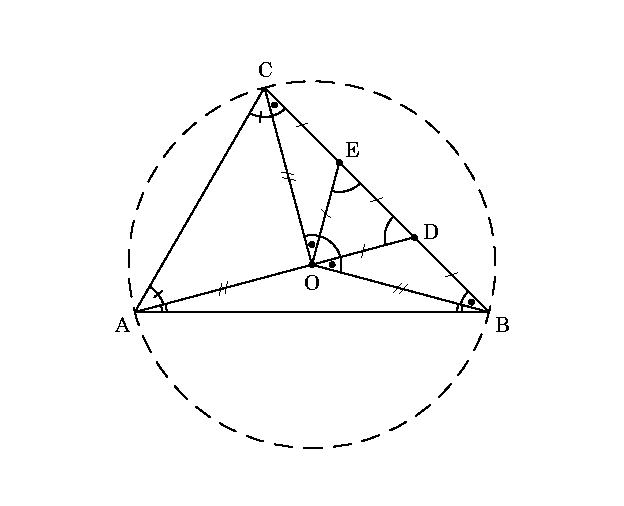
\includegraphics{share/euk/51M04_rmc2007dr071_1.eps}

\begin{claim}
	Si $\triangle{ABC}$ es acutángulo entonces $\angle{ABC} = \ang{45}$, $\angle{ACB} = \ang{75}$, $\angle{CAB} = \ang{60}$.
\end{claim}
\textit{Proof}
En este caso $O$ es interior al $\triangle{ABC}$. Por tal razón

\begin{equation} \label{eq_51M04_rmc2007dr071_19a}
	\angle{ABC} = \angle{OBC} + \angle{OBA}
\end{equation}
\begin{equation} \label{eq_51M04_rmc2007dr071_20}
	\labelcref{eq_51M04_rmc2007dr071_4} \vdash \angle{OAB} + \angle{OBA} = \angle{BOD}
\end{equation}
\begin{equation} \label{eq_51M04_rmc2007dr071_21}
	\labelcref{eq_51M04_rmc2007dr071_19}, \labelcref{eq_51M04_rmc2007dr071_20}, \labelcref{eq_51M04_rmc2007dr071_18} \vdash \angle{OAB} = \angle{OBA} = \ang{15}
\end{equation}
\begin{equation} \label{eq_51M04_rmc2007dr071_22}
	\labelcref{eq_51M04_rmc2007dr071_19a}, \labelcref{eq_51M04_rmc2007dr071_21}, \labelcref{eq_51M04_rmc2007dr071_18}, \labelcref{eq_51M04_rmc2007dr071_4} \vdash \angle{ABC} = \ang{45}
\end{equation}
\begin{equation} \label{eq_51M04_rmc2007dr071_23}
	\labelcref{eq_51M04_rmc2007dr071_19c}, \labelcref{eq_51M04_rmc2007dr071_1}, \labelcref{eq_51M04_rmc2007dr071_2} \vdash \angle{BAC} = \ang{60}
\end{equation}
\begin{equation} \label{eq_51M04_rmc2007dr071_24}
	\labelcref{eq_51M04_rmc2007dr071_0}, \labelcref{eq_51M04_rmc2007dr071_22}, \labelcref{eq_51M04_rmc2007dr071_23} \vdash \angle{BCA} = \ang{75}
\end{equation}

\hfill $\square$

\includegraphics{share/euk/51M04_rmc2007dr071_2.eps}

\begin{claim}
	Si $\triangle{ABC}$ es obtuságulo entonces $\angle{ABC} = \ang{45}$, $\angle{ACB} = \ang{15}$, $\angle{CAB} = \ang{120}$.
\end{claim}
\textit{Proof}
En este caso $O$ es exterior al $\triangle{ABC}$. Por tal razón.

\begin{equation} \label{eq_51M04_rmc2007dr071_25}
	\labelcref{eq_51M04_rmc2007dr071_19c}, \labelcref{eq_51M04_rmc2007dr071_1}, \labelcref{eq_51M04_rmc2007dr071_2} \vdash \overarc{BAC} = \ang{120}
\end{equation}
\begin{equation} \label{eq_51M04_rmc2007dr071_26}
	\labelcref{eq_51M04_rmc2007dr071_25}, \labelcref{eq_51M04_rmc2007dr071_1}, \labelcref{eq_51M04_rmc2007dr071_2} \vdash \angle{BAC} = \ang{120}
\end{equation}
\begin{equation} \label{eq_51M04_rmc2007dr071_27}
	\labelcref{eq_51M04_rmc2007dr071_1}, \labelcref{eq_51M04_rmc2007dr071_2} \vdash \angle{ACB} = \frac{\angle{AOB}}{2}
\end{equation}
\begin{equation} \label{eq_51M04_rmc2007dr071_28}
	\labelcref{eq_51M04_rmc2007dr071_27}, \labelcref{eq_51M04_rmc2007dr071_18}, \labelcref{eq_51M04_rmc2007dr071_4} \vdash \angle{ACB} = \ang{15}
\end{equation}
\begin{equation} \label{eq_51M04_rmc2007dr071_29}
	\labelcref{eq_51M04_rmc2007dr071_0}, \labelcref{eq_51M04_rmc2007dr071_26}, \labelcref{eq_51M04_rmc2007dr071_28} \vdash \angle{ACB} = \ang{45}
\end{equation}

\hfill $\square$

\vspace{1cm}
Lo que queda demostrado. \\\\\\
